%%%% ijcai09.tex

\typeout{IJCAI-09 Instructions for Authors}

% These are the instructions for authors for IJCAI-09.
% They are the same as the ones for IJCAI-07 with superficical wording
%   changes only.

\documentclass{article}
% The file ijcai09.sty is the style file for IJCAI-09 (same as ijcai07.sty).
\usepackage{ijcai09}

% Use the postscript times font!
\usepackage{times}
\usepackage{booktabs}
\usepackage{calc}
\usepackage{enumitem}
\usepackage{graphicx}
\usepackage{microtype}
\usepackage{tabularx}
\usepackage{url}
\usepackage[table]{xcolor}
\usepackage{xspace}
% the following package is optional:
%\usepackage{latexsym} 

% Following comment is from ijcai97-submit.tex:
% The preparation of these files was supported by Schlumberger Palo Alto
% Research, AT\&T Bell Laboratories, and Morgan Kaufmann Publishers.
% Shirley Jowell, of Morgan Kaufmann Publishers, and Peter F.
% Patel-Schneider, of AT\&T Bell Laboratories collaborated on their
% preparation.

% These instructions can be modified and used in other conferences as long
% as credit to the authors and supporting agencies is retained, this notice
% is not changed, and further modification or reuse is not restricted.
% Neither Shirley Jowell nor Peter F. Patel-Schneider can be listed as
% contacts for providing assistance without their prior permission.

% To use for other conferences, change references to files and the
% conference appropriate and use other authors, contacts, publishers, and
% organizations.
% Also change the deadline and address for returning papers and the length and
% page charge instructions.
% Put where the files are available in the appropriate places.

\title{Classifying Controversial Wikipedia Articles}
\author{Ephraim Kunz, Luke Dickinson, Alexandra Hurst, Peter Strein \\
Department of Computer Science\\
Brigham Young University}

\begin{document}

\maketitle

\begin{abstract}
Wikipedia currently has 1300 articles classified as controversial. We examined features and text of both the controversial articles and approximately 1300 other randomly-chosen Wikipedia articles that we deemed non-controversial to attempt to discover what elements of an article make it controversial. We found that running Random Forest on our metadata feature set using 800 trees classified 77\% correctly, while using the text of each Wikipedia article in a Support Vector Machine classified the articles in our dataset with 90\% accuracy. 
\end{abstract}

\section{Introduction}

Some topics and subjects are more sensitive than others. Some topics create an emotional response. Others create an intellectual response. Often people have differing views, and express these views through means of violence. These topics are considered controversial. 

Wikipedia is a source of information publicly available to anyone. Anyone can view and edit this information. Because anyone can change information, edit wars between opposing viewpoints are common for a controversial article. Marking an article as controversial allows readers to be more cautious and moderators to know which articles should be regulated.

We wanted to know if Wikipedia articles could be classified as controversial or non-controversial with machine learning.  It is usually easy for a human to detect an article that is a controversial topic, because we are human, have human emotions, and know from past history what topics tend to be controversial. However as Wikipedia has 5,607,695 English articles \cite{sizeOfWiki} and many more articles in other languages, it becomes impossible to read through all articles to classify them as controversial or not. Thus, a machine learning model that can classify Wikipedia articles could be generalized to work with many different kinds of articles. 

\section{Methodology}

\subsection{Data Sources}

We began the project by collecting a large corpus of raw, labelled data. Wikipedia provides a web API to access their pages, as well as various metadata about a page \cite{apiMain}, such as image urls, links to other pages, inbound links to a page, and categories to which a page belongs. 

\subsection{Initial Data Scrape}

We first scraped the approximately 1300 articles listed on the Wikipedia page “List of controversial issues” \cite{controversialPages}, labelling them as controversial. These are articles identified by Wikipedia’s editors as controversial due to edit warring or lack of a neutral point of view. We then scraped another 1300 articles at random, using a random article endpoint provided by Wikipedia. We labelled all of these articles non-controversial. We wanted a even split between the number controversial and non-controversial articles in order to avoid overfitting on a majority class.

For this raw data scrape, we collected every raw feature available from the Wikipedia API so we could extract meaningful features later. We collected the entire text of each article, the timestamps of every edit ever made to the article and several lists of links (inbound from other Wikipedia pages, outbound to other Wikipedia pages, image urls, and all urls referenced by the article). The sheer amount of data collected made scraping difficult. We wrote a scraper that used rate-limiting and retries to avoid overwhelming Wikipedia and periodically dumped scraped data to files to checkpoint in case of failures. Total, we collected 948 MB of textual data from this first scrape.

\subsection{Data Set}

The raw data collected from the initial scrape was then transformed into several features: percentage of links that were .net, .org, .com, .gov, and other; number of edits; number of words in an article; number of links in an article; number of references; and number of positive/negative/controversial connotation words.  Each instance included these features and an output class of whether it was controversial or not. An actual instance from this dataset is in Table 1.

\begin{table}[ht]

	\centering % used for centering table
	\begin{tabular}{l r}

		Attribute name and type & Attribute value \\ [0.5ex] % inserts table
		%heading
		\hline % inserts single horizontal line
		Net\textunderscore percentage (Continuous) & 0  \\
		Org\textunderscore percentage (Continuous) & 0.0428571  \\
		Avg\textunderscore revisions\textunderscore per\textunderscore day (Continuous) & 0.7883587  \\
		Num\textunderscore links\textunderscore in (Continuous) & 921  \\
		Num\textunderscore controversial\textunderscore words (Continuous) & 1  \\
		Gov\textunderscore percentage (Continuous) & 0.0035714  \\
		Num\textunderscore negative\textunderscore words (Continuous) & 73  \\
		Num\textunderscore images (Continuous) & 20  \\
		Com\textunderscore percentage (Continuous) & 0.2964285  \\
		Article\textunderscore age\textunderscore in\textunderscore days (Continuous) & 4862  \\
		Num\textunderscore revisions (Continuous) & 3833  \\
		Edu\textunderscore percentage (Continuous) & 0  \\
		Num\textunderscore links\textunderscore out (Continuous) & 404  \\
		Other\textunderscore percentage (Continuous) & 0.6571428  \\
		Num\textunderscore categories (Continuous) & 46  \\
		Num\textunderscore positive\textunderscore words (Continuous) & 149  \\
		Num\textunderscore words (Continuous) & 62671  \\
		Num\textunderscore references (Continuous) & 280  \\
		IsControversial (Nominal) & yes  \\
		\hline %inserts single line
	\end{tabular}
	\label{table:nonlin} % is used to refer this table in the text
	\caption{ An example instance of our metadata feature set} % title of Table
\end{table}


We also created a few features to try and capture word bias. These features were num\textunderscore positive\textunderscore words, num\textunderscore negative\textunderscore words, and num\textunderscore controversial\textunderscore words. To obtain these features, we found online lists of words that had a positive connotation \cite{positiveWords}, a negative connotation \cite{negativeWords}, or that were controversial \cite{contraWords}. We then read the body of the Wikipedia article and simply made counts of how many times words from those respective lists appeared.
In the instance above, out of the 62,671 words in the body of the article, 149 had a positive connotation, 73 were considered to be negative, and 1 word was considered to be controversial. 

\subsection{Binned Word Scrape}

Our first scrape yielded 1287 controversial articles and 1325 random articles from Wikipedia which we labeled as non-controversial. However, we learned that by choosing truly random articles, we introduced an unintended bias. Article length became a strong indicator because a large number of our non-controversial articles were short and our controversial articles were long (see results for more details). This made it too easy to detect controversial articles: every long article was categorized as controversial (See Figure 1). We decided that we needed to recollect data so that the controversial articles and the non-controversial articles came from the same distribution of article length. 

%\begin{figure*}
%	\centering
%	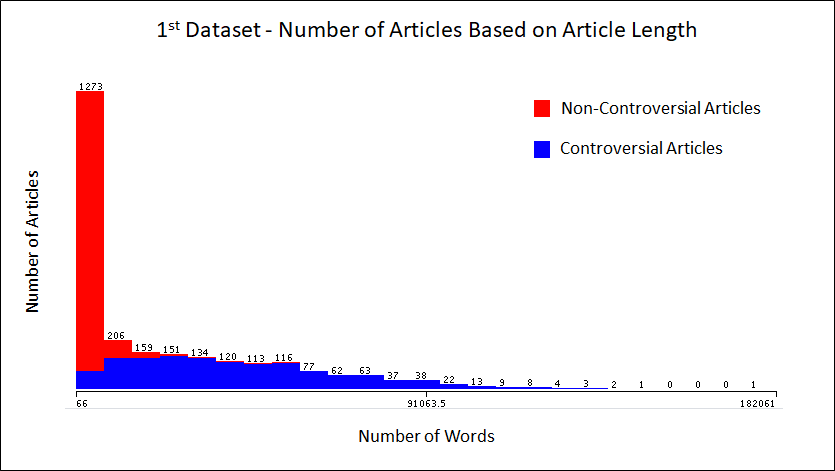
\includegraphics[width=\textwidth]{images/first-scrape.png}
%	\caption{The distribution of articles based on article length of our first date scrape}
%	\label{fig:first-scrape-big}
%\end{figure*}

\begin{figure}[t]
	\centering
	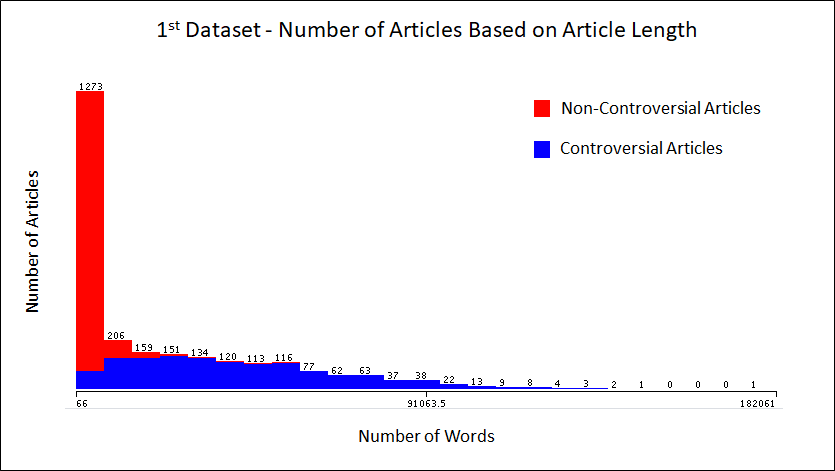
\includegraphics[width=\columnwidth]{images/first-scrape.png}
	\caption{The distribution of articles based on article length of our first date scrape}
	\label{fig:first-scrape}
\end{figure}

To do this, we still used the random article endpoint. This time, however, we created 14 bins based on article length. This allowed us to determine a maximum number of articles to collect for each length category. Scraping took much longer this time, as we had to try many times to randomly receive a longer article. It took longer than 24 hours with multiple scrape processes running.

The distribution of this second dataset is shown in Figure 2. The graph shows that the distributions of articles based on length between the controversial and the non-controversial articles was fairly even.

%\begin{figure*}
%	\centering
%	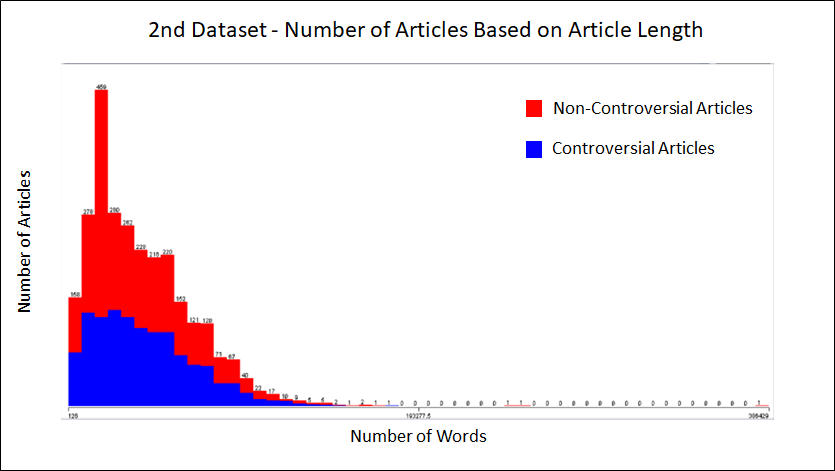
\includegraphics[width=\textwidth]{images/second-scrape.png}
%	\caption{The distribution of articles based on article length of our second date scrape}
%	\label{fig:second-scrape-big}
%\end{figure*}

\begin{figure}[t]
	\centering
	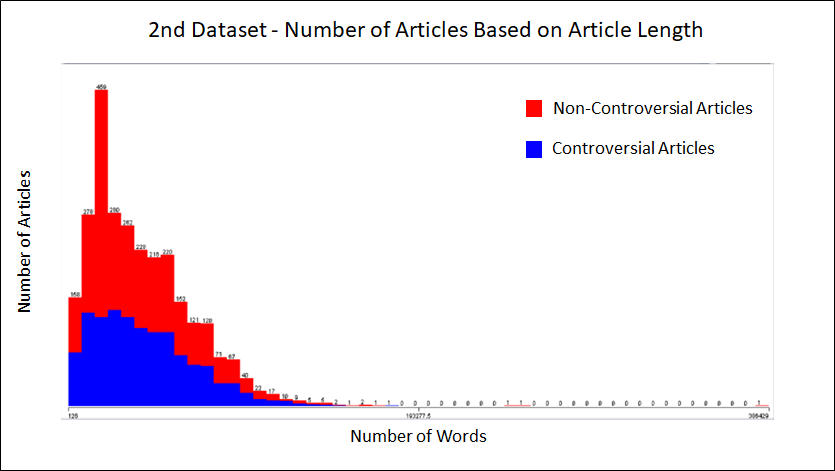
\includegraphics[width=\columnwidth]{images/second-scrape.png}
	\caption{ The distribution of articles based on article length of our second date scrape}
	\label{fig:second-scrape}
\end{figure}

For our second dataset, we collected a total of 2750 articles, 1252 controversial and 1498 non-controversial articles. We collected the same features as used in our first dataset.

\subsection{Bag of Words Dataset}

We also decided to try a machine-learning approach based solely on the text of the article, without other article metadata. We used a bag-of-words approach to construct a dataset. Each article was loaded into Python as one row in a matrix, which was then converted to a numeric array where each column represented the word count of a specific word in each different article. We also used the function TfidfTransform in our sklearn pipeline to make sure common words such as “and,” “the,” and “or” didn’t carry too much weight. From there, our newly-formatted numeric data was ready for use with Python’s sklearn algorithms.

\section{Results}

\subsection{First Dataset}

Before realizing our first dataset was skewed (see Binned Word Scrape), we used it with Weka’s J48 tree and MLP. With J48 we achieved an accuracy of 93.72\% and with MLP we achieved an accuracy of 93.26\%. We believed that this high accuracy was because we were including the number of revisions, a major factor Wikipedia uses to determine if something is controversial. We decided to remove the number of revisions, hoping to get a more reasonable answer. However, we still obtained surprisingly high results. With the J48 tree we obtained 92.38\% accuracy using 10-fold cross validation. With the MLP, we obtained an accuracy of 93.26\% using 10-fold cross validation. These results were still surprisingly high, so we looked more deeply into our data. This led to the discovery of skewing on word length.

\subsection{Second Dataset}
Using the re-scraped data that was no longer skewed, we re-ran the J48 decision tree and the MLP. When we included the number of edits, our accuracies were 75.96\% and 76.04\% respectively. When we excluded the number of edits, our accuracies dropped to 70.44\% and 70.25\% respectively. We concluded that our word length bias was removed and proceeded to further tune these models and our dataset.

Because we had 16 features with a relatively small dataset of only a few thousand instances, we expected to improve our accuracy using MLP by reducing our feature set (curse of dimensionality). We attempted to use Weka’s PCA implementation to combine and reduce our feature set. All of our attempts using PCA only lowered our accuracy.

In another attempt to improve our accuracy, we used Weka’s implementation of random forest to get good results in a tree-based approach to prediction. Trees are beneficial because they make it easier to understand which features are most important and how they are used. In other words, they give us insight into the generalization process of the model. Random forest is an ensemble method. A configurable number of trees are constructed. Each tree is given a random subset of the training set, and it picks a random feature from that subset for each split in the tree. Once all the trees are constructed, the test set is fed to each of them. For each instance in the test set, the vote of all the random trees is taken to determine the predicted output value.

There are many parameters to tune that can be used to improve the performance of random forest for a given dataset. Our initial accuracy with the default settings was 75.94\%, up significantly from our previous best accuracy of 70.44\% with a single tree (no ensemble). After trying out different model parameters, we were able to increase our accuracy to 76.73\% with the random forest. This final model had 800 trees in the forest, broke ties randomly when several attributes looked equally good, and used a bag size of 100\% of the training set. With eight cores being utilized, 10-fold cross validation took 16.2 seconds.

To further improve accuracy, we also improved our positive/negative word counts. We used regular expressions to better separate words in the body text of an article. After improving the word counts, our accuracy using the same random forest model described above increased to 77.38\%.

\subsection{Bag-of-Words, SVM, and Text Analysis}

We used our our bag of words dataset to train models to predict controversy based solely on the text of an article. We used both Naive Bayes and Support Vector Machines.

Support Vector Machines (SVM) are classifiers suited well to high dimensional or nonlinear data. We used this method with our bag-of-words data. When we originally tried text classification using Naive Bayes classification, our accuracy was only around 65\%, so SVMs offered a similar classification technique that might work better with what appeared to be nonlinear data. Our results were promising. Average classification accuracy using an 80-20 split yielded 90\% accuracy on average. A histogram of accuracies over 25 runs of the algorithm is shown in Figure 3.

\begin{figure}[t]
	\centering
	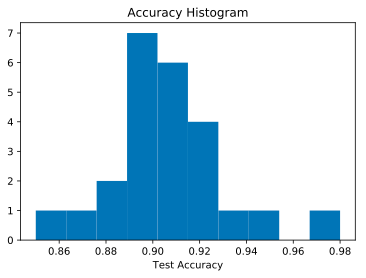
\includegraphics[width=\columnwidth]{images/svm.png}
	\caption{An accuracy comparison of 25 Support Vector Machine experiments using the body text of articles as a feature set}
	\label{fig:svm}
\end{figure}

To ensure the legitimacy of our results and to easily compare the results of our random forest and SVM models, we created five standard sets from our data with a 80/20 test/training split. The results are shown in Table 2. 

\begin{table}[ht]
	
	\centering % used for centering table
	\begin{tabular}{l l l}
		
		Dataset & Random Forest & Support Vector Machine \\ [0.5ex] % inserts table
		%heading
		\hline % inserts single horizontal line
		1 & 76.15\% & xx.xx\% \\
		2 & 74.82\% & xx.xx\%  \\
		3 & 78.80\% & xx.xx\% \\
		4 & 79.09\% & xx.xx\% \\
		5 & 76.59\% & xx.xx\% \\
		Average & 77.09\% & xx.xx\%  \\
		\hline %inserts single line
	\end{tabular}
	\label{table:compare} % is used to refer this table in the text
	\caption{ An accuracy comparison of a cross validation experiment using 80\% training set and 20\% test set using Random Forest and Support Vector Machine} 
\end{table}


Additionally, we experimented with Latent Dirichlet Allocation and Non-Negative Matrix Factorization, algorithms that find key words or ideas in articles, to try to highlight phrases that may lead to an algorithm being classified as controversial. While most of these efforts mostly produced a list of “of,” “thus,” and “in,” several controversial words like “sex” or “rock” showed up multiple times. Dates also seemed to show up more in controversial articles. Though the LDA and NMF efforts didn’t produce any strong results, they highlighted some of the efforts of Support Vector Machines in trying to figure out what text elements lead to a controversial document.

\section{Conclusion and Future Work}
We conclude that analyzing the text of a Wikipedia article was more indicative of controversy than the features of Wikipedia. With the random forest model, we achieved an accuracy of 77.38%. However, when we used a bag-of-words feature set with SVM as the model, we achieved an average accuracy of 90%. If we had more time, we would pursue more methods that better analyze text than bag-of-word approaches. 

We also discovered that there is no one feature that was indicative of controversy. It was a combination of higher order features that enabled us to get the best results. If we had more time, we would examine what articles are being misclassified, and why they are being misclassified. Were there any features in common? Were there similarities between which articles our random forest got wrong and which the SVM got wrong? These are all questions we would like to explore. 

One problem we ran into was the small dataset. Because Wikipedia already classified 1300 articles as controversial, we could use those articles as a base. However, we could not expand our dataset to include more than 2600 articles because we did not want our program to overfit on the majority class. We would like to explore bootstrapping our data so that we could get more data to train our models. Then we could train our model on all Wikipedia articles.

Classifying controversial articles is essentially an outlier problem. There are over 5 million Wikipedia articles on Wikipedia, but only 1300 articles are classified as controversial. This means that finding controversial articles is the same as trying to find a few outliers in a giant dataset. If we had more time, we would research more ways to detect outliers.

We would also further analyze different output classes. It is possible that two output classifications (controversial or non-controversial) are not sufficient for this problem. There may be articles that are not controversial, are kind of controversial, that are very controversial, and that are completely controversial. There may also be other clusters that we are not aware of. Knowing the best clustering of the data would help us to know how to improve the features in our datasets.


\bibliographystyle{named}
\bibliography{main}

\end{document}

